

\tikzset{every picture/.style={line width=0.75pt}} %set default line width to 0.75pt        

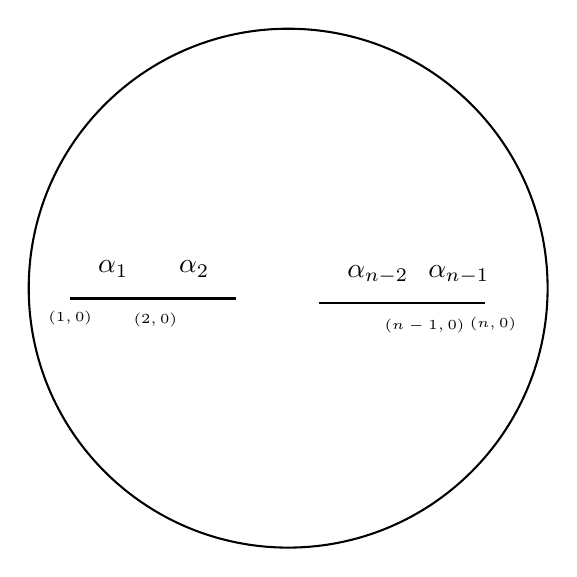
\begin{tikzpicture}[x=0.75pt,y=0.75pt,yscale=-1,xscale=1]
%uncomment if require: \path (0,877); %set diagram left start at 0, and has height of 877

%Shape: Circle [id:dp37495404303702484] 
\draw   (110,145) .. controls (110,75.96) and (165.96,20) .. (235,20) .. controls (304.04,20) and (360,75.96) .. (360,145) .. controls (360,214.04) and (304.04,270) .. (235,270) .. controls (165.96,270) and (110,214.04) .. (110,145) -- cycle ;
%Straight Lines [id:da09124629345358082] 
\draw    (130,150) -- (170,150) ;
%Straight Lines [id:da35678252994237136] 
\draw    (170,150) -- (210,150) ;
%Straight Lines [id:da5587533975361445] 
\draw    (250,152) -- (290,152) ;
%Straight Lines [id:da14803740874356064] 
\draw    (290,152) -- (330,152) ;

% Text Node
\draw (142,130.4) node [anchor=north west][inner sep=0.75pt]    {$\alpha _{1}$};
% Text Node
\draw (181,130.4) node [anchor=north west][inner sep=0.75pt]    {$\alpha _{2}$};
% Text Node
\draw (221,136.4) node [anchor=north west][inner sep=0.75pt]    {$\dotsc $};
% Text Node
\draw (262,132.4) node [anchor=north west][inner sep=0.75pt]    {$\alpha _{n-2}$};
% Text Node
\draw (301,132.4) node [anchor=north west][inner sep=0.75pt]    {$\alpha _{n-1}$};
% Text Node
\draw (118,154.4) node [anchor=north west][inner sep=0.75pt]  [font=\tiny]  {$( 1,0)$};
% Text Node
\draw (159,155.4) node [anchor=north west][inner sep=0.75pt]  [font=\tiny]  {$( 2,0)$};
% Text Node
\draw (280,158.4) node [anchor=north west][inner sep=0.75pt]  [font=\tiny]  {$( n-1,0)$};
% Text Node
\draw (321,157.4) node [anchor=north west][inner sep=0.75pt]  [font=\tiny]  {$( n,0)$};


\end{tikzpicture}
